 \section{Contexto em Sistemas Distribuídos e em Software Livre}

  \begin{frame}{Sistemas de Arquivos Distribuídos}
     \begin{itemize}
      \item<1-> Processar um volume relativamente grande de dados é possível, em poucas horas, com alguns dólares e com algumas máquinas: http://aws.amazon.com/
      \item<2-> Isto também pode ser feito com o Hadoop, um \emph{framework} para processamento de dados em larga escala.
      \item<3-> Volume grande de dados ?
          \begin{itemize}
             \item<4-> megabyte - $10^6$ - uma foto
             \item<5-> gigabyte - $10^9$ - um DVD armazena 4.7 GB de um filme
             \item<6-> terabyte - $10^{12}$ - 200 filmes
             \item<7-> petabyte - $10^{15}$
             \item<8-> exabyte - $10^{18}$
             \item<9-> zettabyte - $10^{21}$ - um disco de 140 GB para cada pessoa no mundo
          \end{itemize}
     \end{itemize}
  \end{frame}

  \begin{frame}{Software Open Source}

% http://feedgrowth.com/idea-categories/social-networking/secure-your-brands-username-and-vanity-url-on-facebook/
   \begin{figure}[hb]
     \centering
     
\includegraphics[scale=0.3]{facebook-logo.jpg}
     
\includegraphics[scale=0.2]{yahoo-logo-300x224.jpg}
     
\includegraphics[scale=1]{google-logo.jpg}
     
\includegraphics[scale=0.06]{new-twitter-logo.jpg}
     
\includegraphics[scale=0.1]{lastfm.jpg}
     
\includegraphics[scale=0.1]{microsoft-logo.jpg}
     
\includegraphics[scale=0.1]{IBM-logo.jpg}
%     \caption{Facebook www.facebook.com}
     \label{fig11:fb}
   \end{figure}

% http://www.scienceweek.ie/features/2012-featured-articles/google-experiments.html
%   \begin{figure}[hb]
%     \centering
%     
\includegraphics[scale=1]{google-logo.jpg}
%     \caption{Facebook www.facebook.com}
%     \label{fig12:goo}
%   \end{figure}

% http://theinspirationroom.com/daily/2012/twitter-logo-redesigned/
%   \begin{figure}[hb]
%     \centering
%     
\includegraphics[scale=0.1]{new-twitter-logo.jpg}
%     \caption{Facebook www.facebook.com}
%     \label{fig13:twi}
%   \end{figure}

% http://www.telegraph.co.uk/technology/microsoft/9495544/Microsoft-unveils-new-logo.html
%   \begin{figure}[hb]
%     \centering
%     
\includegraphics[scale=0.2]{microsoft-logo.jpg}
%     \caption{Facebook www.facebook.com}
%     \label{fig14:ms}
%   \end{figure}

% http://darts.cse.nd.edu/projects/ibm-logo/
%   \begin{figure}[hb]
%     \centering
%     
\includegraphics[scale=0.1]{IBM-logo.jpg}
%     \caption{Facebook www.facebook.com}
%     \label{fig15:ibm}
%   \end{figure}


% http://www.cloudbook.net/directories/research-clouds/university-of-maryland-college-park
% http://creeva.com/2012/03/08/i-have-successfully-merged-last-fm-accounts-here-is-a-howto/
% http://terrierteam.dcs.gla.ac.uk/

   \begin{figure}[hb]
     \centering
     
\includegraphics[scale=1]{CompScience_colour_stk-2.jpg}
     
\includegraphics[scale=0.3]{university_of_maryland_college_park_logo2.jpg}
     
\includegraphics[scale=0.3]{cornell.jpg}
%     \caption{Facebook www.facebook.com}
     \label{fig11:fb}
   \end{figure}

% http://tomcat.apache.org/
   \begin{figure}[hb]
     \centering
     
\includegraphics[scale=0.2]{asf-logo.jpg}
      
\includegraphics[scale=2]{hadoop-logo.jpg}
%     \caption{Facebook www.facebook.com}
     \label{fig16:afs}
   \end{figure}

     \begin{itemize}
        \item<1-> O Hadoop disponibiliza um armazenamento compartilhado (HDFS/Hadoop \emph{Distributed Filesystem}) e um sistema de análise (MapReduce), formando um \emph{framework} ou arcabouço.
%         \item<2-> Facebook, Google, Twitter, Microsoft e IBM armazenam dados do tamanho de petabytes e utilizam o Hadoop.
%         \item<3-> O projeto Hadoop é hoje um projeto independente dentro da hierarquia de projetos da Apache Software Foundation.
     \end{itemize}
  \end{frame}

  \begin{frame}{RDBMS X HDFS/MapReduce}
    Por que não usamos banco de dados ?
     \begin{itemize}
        \item<1->  Em um banco de dados, uma atualização da árvore-B pode gerar muitas operações de \emph{seeking}.
        \item<2->  \emph{seek time} - processo de mover a cabeça do disco para um dado local no disco com o objetivo de ler ou de escrever dados
        \item<3->  É mais rápido usar um algoritmo de ordenação (\emph{sort}/\emph{merge}) para:
          \begin{itemize}
             \item<4-> analisar um grande volume de dados do tamanho de petabytes
             \item<5-> reconstruir toda a base de dados
          \end{itemize}
      \end{itemize}
  \end{frame}

  \begin{frame}{RDBMS X HDFS/MapReduce}
{\small
        \begin{center}
          \begin{tabular}{|p{2cm}||p{3.5cm}||p{3.5cm}|}
            \hline
& Aplicação para RDBMS & Aplicação para HDFS/MapReduce\\ \hline
tamanho & gigabytes & petabytes\\ \hline
acesso & OLTP(interativo) e \emph{batch} & \emph{batch}\\ \hline
atualização & lê e escreve muitas vezes & escreve uma vez, lê muitas vezes\\ \hline
esquema & estático & dinâmico\\ \hline
integridade & alta & baixa\\ \hline
escala & não linear & linear\\ \hline
          \end{tabular}
        \end{center}
}

Fonte: \cite{White:2009}
  \end{frame}

  \begin{frame}{HDFS}

    \begin{figure}[hb]
      \centering
      
\includegraphics[scale=2]{hadoop-logo.jpg}
%      \caption{Projeto Hadoop \cite{Hadoop:2010}}
%      \label{fig5:php}
    \end{figure}

HFS disponibiliza espaço para sistema de arquivos e permite que os dados do usuário sejam armazenados em arquivos. Internamente, um arquivo é dividido em um ou mais blocos e esses blocos são armazenados em um conjunto de DataNodes. O tamanho \emph{default} de cada bloco é 64MB.

    \begin{figure}[hb]
      \centering
      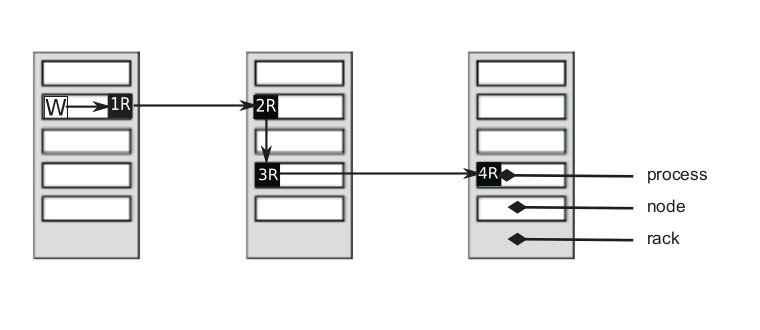
\includegraphics[scale=0.4]{HDFS-arquitetura-replicacao-2.jpg}
      \caption{Arquitetura do HFS - Datanodes e Blocos \cite{Hadoop:2010}}
      \label{fig7:hfs}
    \end{figure} 

  \end{frame}


  \begin{frame}{MapReduce}

    \begin{figure}[hb]
      \centering
      
\includegraphics[scale=2]{hadoop-logo.jpg}
%      \caption{Projeto Hadoop \cite{Hadoop:2010}}
%      \label{fig5:php}
    \end{figure}

     \begin{itemize}
       \item<1-> Os dados que MapReduce processa são dados não estruturados como texto ou imagens. O HDFS, através do \emph{pipeline} dos DataNodes, tenta colocar esses dados no nó onde são feitas as computações, desta forma, o acesso aos dados é rápido, pois é "mais" local.
       \item<2-> O MapReduce pode resolver problemas genéricos cujos dados podem ser divididos em matrizes de dados, para cada matriz a mesma computação é necessária e não existe necessidade de comunicação entre as tarefas.
       \item<3-> Problemas como empacotamento, linha de fábrica, otimização não são resolvidos pelo modelo de computação do MapReduce.
     \end{itemize}

  \end{frame}

  \begin{frame}{MapReduce}

    \begin{figure}[hb]
      \centering
      
\includegraphics[scale=2]{hadoop-logo.jpg}
%      \caption{Projeto Hadoop \cite{Hadoop:2010}}
%      \label{fig5:php}
    \end{figure}

Problema genérico:
\begin{itemize}
   \item iteração sobre um número grande de registros
   \item \emph{Map} extrai algo de cada registro (chave, valor)
   \item rearranjo (\emph{shuffle} e ordenação de resultados intermediários por (chave, valor)
   \item \emph{Reduce} agrega os resultados intermediários 
   \item geração da saída
\end{itemize}

  \end{frame}

